%!TEX root = ../dissertation.tex
% =====================================================================
%  CHAPTER 4 — THE i-CIR BENCHMARK
% ---------------------------------------------------------------------
%  Self-contained description of the problem, the dataset, the metrics,
%  and the BASIC baseline that this thesis builds on.  Written for a
%  committee in which at most one reader has a machine-learning
%  background and none is a computer-vision specialist: every formal
%  object is introduced with a plain-language intuition and a concrete
%  example before any equation.
%
%  Notation (defined in dissertation.tex, i-CIR-aligned):
%   \qv q^v query image | \qt q^t query text | \qc c target caption
%   \DB X database | \xdb x a db image | \encv \enct encoders
%   \simop sim | \clamp clamp | \sv \st \sc the three scores
%
%  Labels are PRESERVED from the chapters this content moved out of
%  (sect:method_problem, sect:method_dataset, sect:method_eval,
%  sect:rel_basic / sect:method_basic, subsect:method_centering, the
%  figures, the tables and the equations) so that cross-references from
%  the other chapters keep resolving automatically.
% =====================================================================

\chapter{The i-CIR Benchmark}\label{chapt:benchmark}

Before a new retrieval method can be proposed, the task it is meant to solve
and the yardstick by which it will be judged must be pinned down precisely.
This chapter does exactly that. It is deliberately self-contained: the method
of Chapter~\ref{chapt:method} is built directly on top of the material presented
here, so a reader who understands this chapter has everything needed to follow
the contribution.

A recurring theme of Chapter~\ref{chapt:related} was that \emph{how} a composed
image retrieval system is evaluated matters at least as much as the system
itself. Many popular benchmarks can be solved by cheating: a model can ignore
either the image or the text and still score well, because the two are
correlated or the alternatives in the gallery are too easy to tell
apart~\cite{attimonelli2026circus}. This thesis therefore evaluates on
i-CIR~\cite{psomas2025icir}, a benchmark engineered specifically to make such
shortcuts fail. The chapter proceeds as follows.
Section~\ref{sect:method_problem} states the composed image retrieval task, fixes
the notation used for the rest of the thesis, and explains the \emph{instance-level}
notion of a correct answer that gives i-CIR its difficulty.
Section~\ref{sect:method_dataset} describes the dataset itself -- how it is built,
how large it is, and what its statistics look like.
Section~\ref{sect:method_eval} defines the evaluation protocol and the metrics
used to turn a ranking into a single comparable number.
Section~\ref{sect:method_basic} presents \textsc{Basic}, the training-free
baseline released with the benchmark, in the full detail required to understand
the method that extends it.

% =====================================================================
\section{Problem Formulation and Notation}\label{sect:method_problem}
% =====================================================================

\paragraph{Composed image retrieval.}
In ordinary image search the query is a single thing: either an example image
(``find more pictures like this one'') or a few words (``find pictures of a red
handbag''). \emph{Composed} image retrieval (CIR) combines the two. A query is a
pair $q = (\qv, \qt)$, where $\qv$ is a reference \emph{query image} and $\qt$ is
a short \emph{query text} that says how the desired result should differ from
$\qv$. For example, the reference image might show a particular handbag and the
text might read \emph{``in red''}; the intended answer is a picture of \emph{that
same handbag, but red}. The modification text is a \emph{relative} instruction --
it only makes sense in the context of the image -- which is precisely what makes
the task hard: the system must read the image to know \emph{what} is being
changed and the text to know \emph{how}, and then combine the two.

Formally, given a database of images $\DB = \{\xdb_1, \dots, \xdb_N\}$, the goal
is to produce a ranking of $\DB$ that places the image the user intends -- the
result of applying the modification $\qt$ to the object shown in $\qv$ -- as
close to the top as possible. As introduced in Chapter~\ref{chapt:background},
we denote by $\encv$ the visual encoder of a frozen vision--language model and by
$\enct$ its textual encoder; both map their input to an $\ell_2$-normalised
vector in a shared $d$-dimensional space, so that an image and a text can be
compared directly by a dot product (their cosine similarity). Throughout, image
similarities and image--text similarities are computed as such dot products.

\paragraph{Instance-level relevance: the source of the difficulty.}
The single most important design choice of i-CIR is what counts as a \emph{correct}
answer. In most earlier benchmarks correctness is defined at the \emph{category}
level: for the query \emph{``a red handbag''}, \emph{any} red handbag is accepted.
i-CIR instead defines correctness at the level of a specific object
\emph{instance}. A retrieved image is relevant only if it depicts the \emph{same
individual object} as the reference image, modified as the text requests -- not
merely another object of the same kind. The everyday analogy is the difference
between ``find me a photo of a dog'' (category) and ``find me another photo of
\emph{my} dog'' (instance): the second is far more demanding, because a
superficially similar but different dog is now a mistake rather than a success.

This instance-level definition is what forces a method to genuinely use
\emph{both} modalities. To make the point unavoidable, the benchmark deliberately
surrounds every query with three kinds of \emph{hard negatives} -- distractor
images that are designed to look correct if the method pays attention to only one
half of the query:
\begin{itemize}
  \item \textbf{Visual hard negatives}: the same or a visually similar instance
        that does \emph{not} satisfy the modification (it fails the text).
  \item \textbf{Textual hard negatives}: images that \emph{do} satisfy the
        modification text but show a \emph{different} instance (they fail the
        image).
  \item \textbf{Composed hard negatives}: the correct instance under a
        \emph{different} modification (they satisfy the image and are on-topic,
        but apply the wrong change).
\end{itemize}
Figure~\ref{fig:icir_query} lays out this structure schematically. A method that
collapses onto a single modality is systematically trapped: relying on the image
alone promotes the visual and composed negatives, while relying on the text alone
promotes the textual negatives. Only a method that respects the visual identity
of the instance \emph{and} applies the precise change demanded by the text can
separate the true target from its look-alikes.

\begin{figure}[htbp]
  \centering
  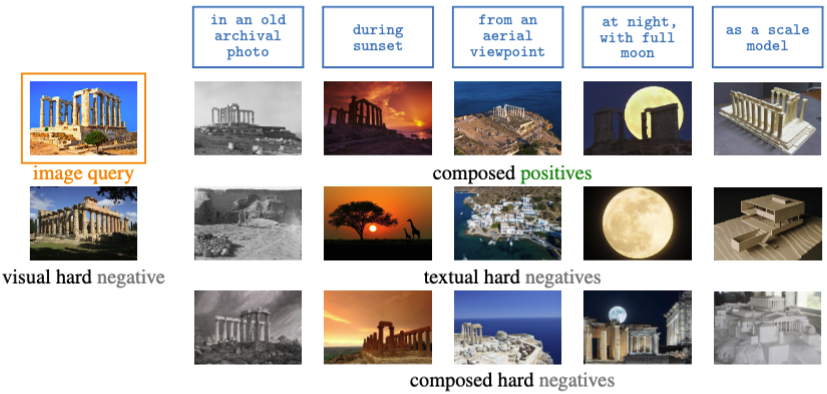
\includegraphics[width=\linewidth]{figures/icir_dataset}
  \caption{%
    Structure of an i-CIR query. Given a reference (query) image and a
    modification text, the retrieval pool contains the correct target
    (a \emph{composed positive}) together with the three types of hard
    negatives: \emph{visual} (same instance, different modification),
    \emph{textual} (different instance, correct modification), and
    \emph{composed} (different instance, different modification). The
    pool is arranged so that no single modality is enough to find the
    answer. Reproduced from Psomas~et~al.~\cite{psomas2025icir}.%
  }
  \label{fig:icir_query}
\end{figure}

The pattern in Figure~\ref{fig:icir_query} is not a
special case engineered around a single instance: it recurs across every kind of
object the benchmark covers. Figure~\ref{fig:icir_category_examples} shows eight
further examples spanning strikingly different visual and textual categories --
a gold death mask repainted as art, a sneaker with swapped shoelaces, the
Leaning Tower seen from the air, a chocolate bunny turned into an outdoor
installation, a cartoon rat placed on a mug, a decorative duck moved into a
garden, a muscle car reimagined as a cabrio, and a film camera fitted with an
external flash -- each accompanied by its own visual, textual, and composed
hard negative. The three-negative structure, and the need to read the image and
the text together, is therefore a property of the benchmark's design, not an
artefact of any single category.

\begin{figure}[htbp]
  \centering
  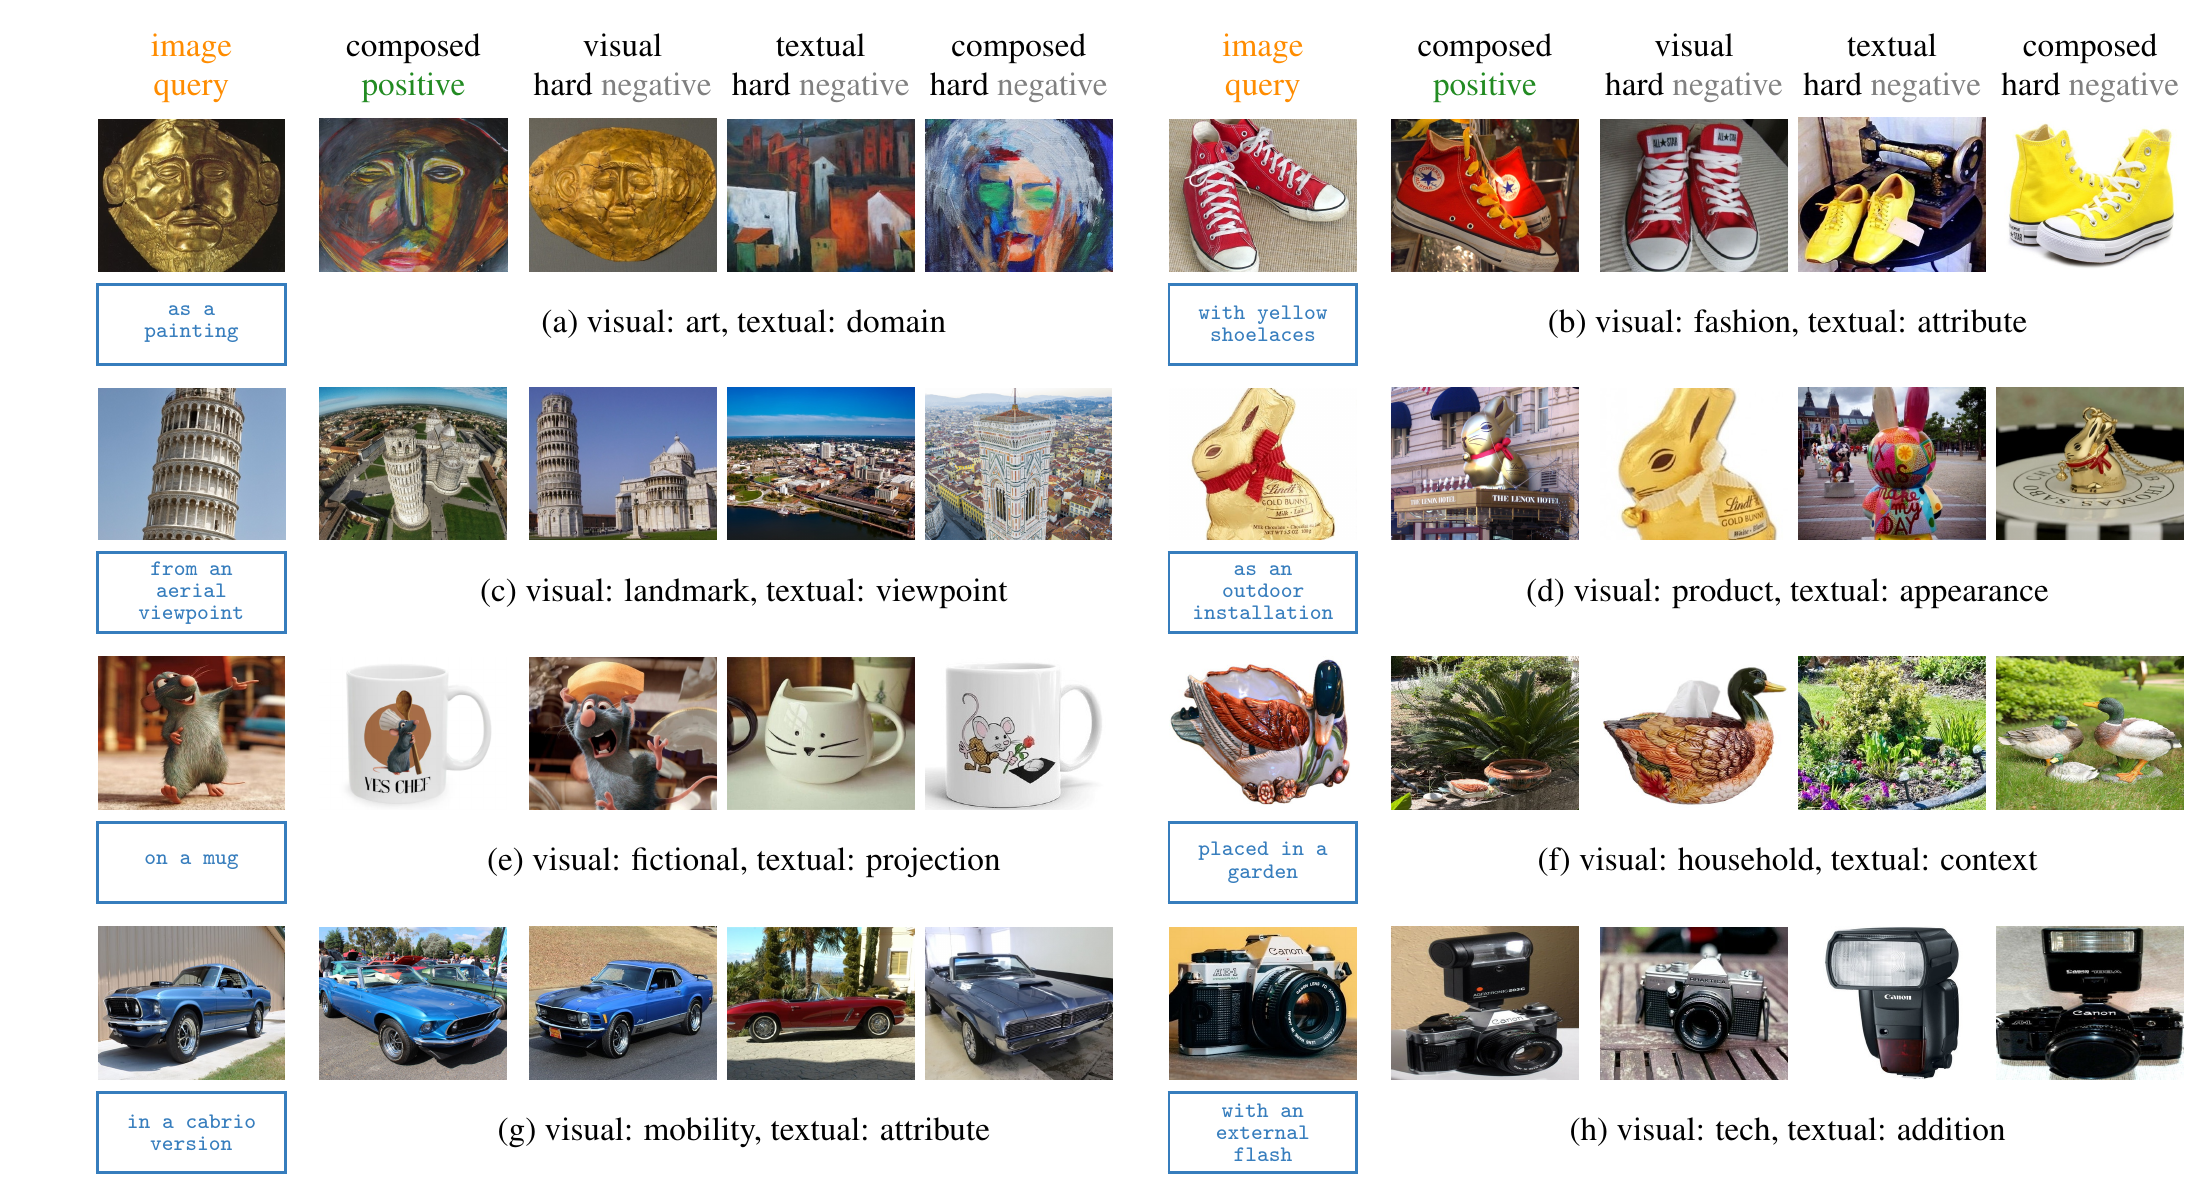
\includegraphics[width=\linewidth]{figures/icir_category_examples}
  \caption{%
    Visualization of visual and textual category examples from i-CIR. For each
    of eight randomly chosen category pairings (a--h), the image query, the
    text query, the composed positive, the visual hard negative, the textual
    hard negative, and the composed hard negative are shown. Reproduced from
    Psomas~et~al.~\cite{psomas2025icir}.%
  }
  \label{fig:icir_category_examples}
\end{figure}

\paragraph{Zero-shot assumption.}
This thesis operates strictly in the \emph{zero-shot} regime: no component of the
system is ever trained or fine-tuned on i-CIR. All encoders $\encv, \enct$ are
off-the-shelf, frozen vision--language models (Chapter~\ref{chapt:background}),
the caption generator of Chapter~\ref{chapt:method} is a frozen multimodal model,
and every fusion and post-processing step is training-free. This choice is not a
limitation but a deliberate stance, for three reasons:
\begin{itemize}
  \item \textbf{Supervised training is expensive and labour-intensive.} It
        requires large collections of annotated triplets -- reference image,
        modification text, and the correct target image -- which are costly and
        slow to gather.
  \item \textbf{It does not scale.} Building a dedicated training set for every
        kind of modification a user might ever request is unrealistic; the space
        of possible edits is effectively open-ended.
  \item \textbf{Trained models generalise poorly.} A fusion model trained on one
        CIR dataset typically transfers badly to another, so the effort must be
        repeated for each new domain.
\end{itemize}
Operating zero-shot side-steps all three issues. It also has a scientific
benefit specific to this study: because nothing is trained on the benchmark, any
measured improvement can be attributed to the proposed retrieval \emph{signal}
itself, and not to the model having memorised the evaluation data.

% =====================================================================
\section{The i-CIR Dataset}\label{sect:method_dataset}
% =====================================================================

We conduct all experiments on i-CIR~\cite{psomas2025icir}, the instance-level
composed image retrieval benchmark. This section describes how the dataset is
organised, how large it is, and what its statistics reveal about the retrieval
problem it poses.

\paragraph{How the dataset is organised.}
The benchmark is built around $202$ distinct object \emph{instances}. An instance
is one specific thing -- a particular landmark (the \emph{Temple of Hephaestus}),
a particular product (a specific model of trainer), or a specific character
(\emph{Homer Simpson}). Each instance comes with one or more reference images and
a set of modification texts that make sense for it; pairing a reference image with
a modification text yields a composed query. On the database side, every instance
owns a folder tree of the following shape:
\begin{center}
\ttfamily database / \{instance\} / \{modification\} / \dots\ positive images \dots
\end{center}
so that for each modification of an instance there is a small folder holding the
\emph{positive} (correct) target images, plus one large \texttt{hn/} folder of
curated \emph{hard-negative} images for that instance. The ground truth of a query
is therefore defined purely by folder membership: an image is relevant to the
query $(\text{instance}, \text{modification})$ exactly when it lives in that
instance's folder for that modification.

\paragraph{Instance diversity.}
Figure~\ref{fig:icir_instances_grid} gives a bird's-eye view of the benchmark,
showing one randomly sampled query image for each of the $202$ instances. The
collage makes concrete how broad ``instance'' is meant to be: landmarks
(the Colosseum, the Parthenon), fictional characters (Mickey Mouse, Luffy),
vehicles, household objects, fashion items, toys, and consumer products all sit
side by side. This heterogeneity matters for the argument of
Section~\ref{sect:method_problem}: because instances are drawn from so many
unrelated domains, a method cannot rely on domain-specific priors and must
instead genuinely read the reference image and the modification text for every
query.

\begin{figure}[p]
  \centering
  \includegraphics[width=0.85\linewidth,height=0.82\textheight,keepaspectratio]{figures/icir_instances_grid}
  \caption{%
    The $202$ instances of i-CIR. A query image is randomly sampled per object
    instance. Reproduced from Psomas~et~al.~\cite{psomas2025icir}.%
  }
  \label{fig:icir_instances_grid}
\end{figure}

\paragraph{Category taxonomy.}
To organise this diversity, i-CIR defines two complementary taxonomies, shown in
Figure~\ref{fig:icir_taxonomy}. Visual categories are arranged in a $3$-level
hierarchy (for instance \emph{household} $\to$ \emph{kitchenware} $\to$
\emph{mug}), while textual modification categories are labelled at a single
level (\emph{projection}, \emph{domain}, \emph{attribute}, \emph{appearance},
\emph{viewpoint}, \emph{addition}, \emph{context}). Beyond documenting the
benchmark's coverage, this taxonomy is what makes the category-pairing view of
Figure~\ref{fig:icir_category_examples} possible in the first place, and it
enables performance to be reported per category rather than only in aggregate.

\begin{figure}[p]
  \centering
  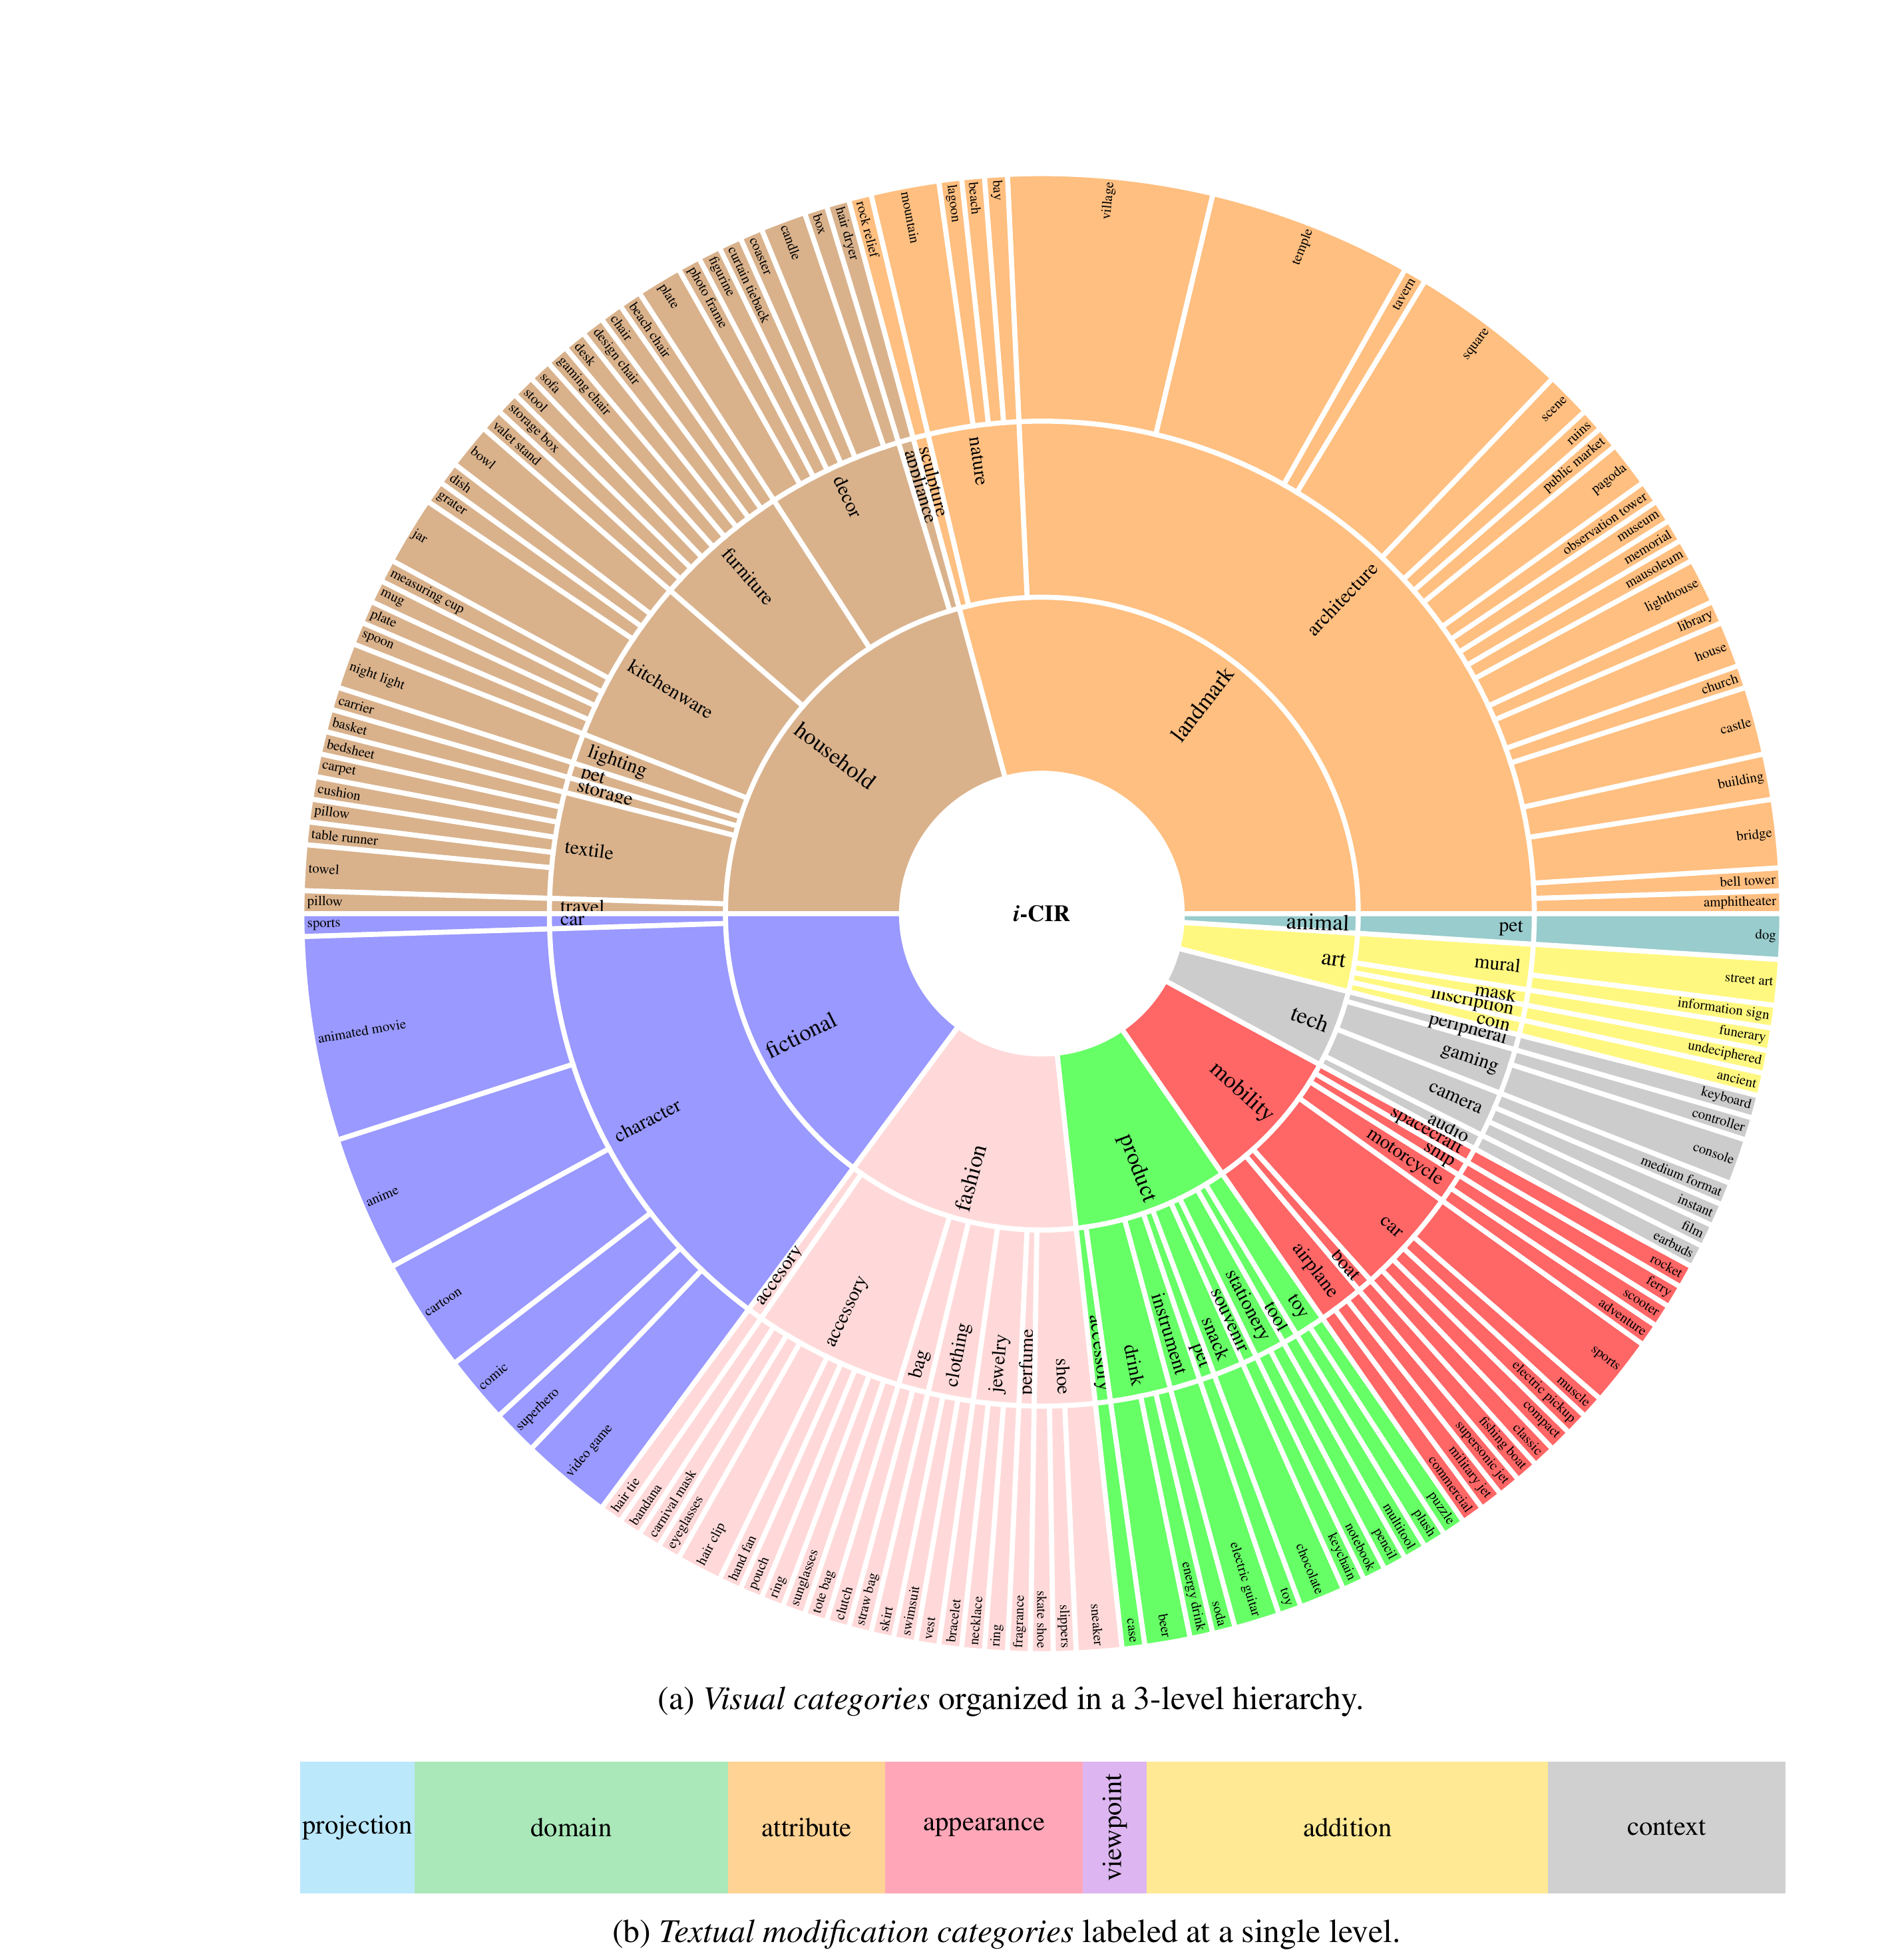
\includegraphics[width=0.85\linewidth,height=0.82\textheight,keepaspectratio]{figures/icir_taxonomy}
  \caption{%
    The i-CIR taxonomies showing (a) the $3$-level hierarchy of visual
    categories and (b) the single-level taxonomy of textual modification
    categories. This taxonomy captures the diversity and distribution of
    object instances and textual queries, and enables performance reporting
    per category. Reproduced from Psomas~et~al.~\cite{psomas2025icir}.%
  }
  \label{fig:icir_taxonomy}
\end{figure}

\paragraph{Query-specific instance pool.}
Rather than ranking every query against all $752{,}092$ images at once, i-CIR
evaluates each query inside a dedicated \emph{pool}: the set of images belonging
to the query's own instance. This pool gathers the positive images of every
modification of that instance together with the instance's large collection of
hard negatives -- exactly the visual, textual, and composed distractors of
Section~\ref{sect:method_problem}. Concentrating closely related look-alikes
around each query is what makes the ranking task hard: the method is not asked to
tell a temple apart from a teapot, but to tell the \emph{right} temple, under the
\emph{right} modification, apart from dozens of near-misses.

\paragraph{Scale.}
The full benchmark comprises $1{,}883$ composed queries built from $695$ distinct
reference images and $334$ distinct modification texts, over the $202$ instances,
with a total of $N = 752{,}092$ database images. Instance pools are large: they
range from about one thousand to roughly ten thousand images (median $3{,}435$),
so even a single query is a search over thousands of deliberately confusing
candidates. For development we additionally use a fixed $20\%$ instance subset
($400$ queries; see Section~\ref{sect:method_impl}), on which the ablation studies
of Chapter~\ref{chapt:results} are conducted; the headline results are always
reported on the full benchmark.

\paragraph{What the statistics say.}
Figure~\ref{fig:icir_stats} summarises the shape of the benchmark and reinforces
why it is challenging. Three features stand out.
\emph{First}, the positive set of a query is tiny
(Figure~\ref{fig:icir_stats}b): a query has a median of only $5$ correct images,
and half of all queries have fewer than that, hidden among thousands of pool
images. There is very little room for error -- the correct answers must land at
the very top of the ranking to score well.
\emph{Second}, the modification texts are extremely short
(Figure~\ref{fig:icir_stats}d): a median of $4$ words, and often only one or two
(\emph{``at night''}, \emph{``as a sketch''}). Such fragments carry little
standalone meaning, which -- as later sections show -- is the crux of the
difficulty on the text side and the opening this thesis exploits.
\emph{Third}, the modifications are genuinely open-domain
(Figure~\ref{fig:icir_stats}e): the most common edits ask to re-imagine an object
as an action figure, on a t-shirt, at night, as a statue, or from the air -- edits
that change the object's appearance drastically while preserving its identity,
which is exactly what a category-level system cannot handle. The number of queries
per instance is itself uneven (Figure~\ref{fig:icir_stats}a; median $6$, but up to
$48$), a skew that motivates the choice of averaging protocol in
Section~\ref{sect:method_eval}.

\begin{figure}[htbp]
  \centering
  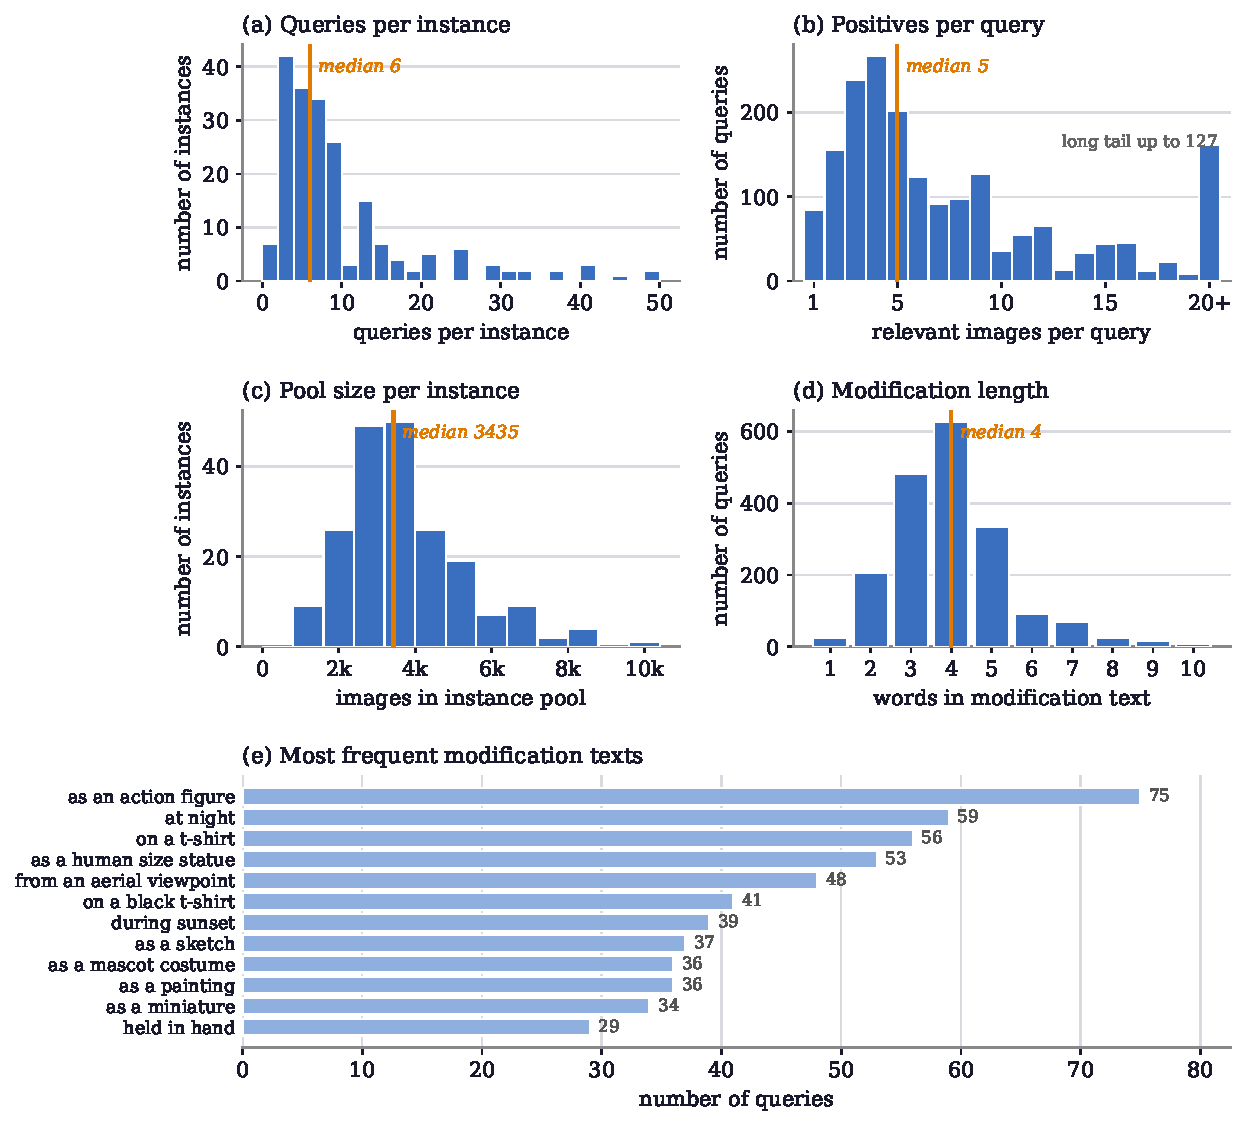
\includegraphics[width=\linewidth]{figures/icir_stats}
  \caption[Statistics of the i-CIR benchmark.]{%
    Statistics of the i-CIR benchmark ($202$ instances, $1{,}883$ queries,
    $752{,}092$ images). \textbf{(a)}~queries per instance (median $6$);
    \textbf{(b)}~relevant images per query (median $5$, with a long tail up to
    $127$); \textbf{(c)}~size of each instance's retrieval pool (median
    $3{,}435$ images); \textbf{(d)}~length of the modification text in words
    (median $4$); \textbf{(e)}~the most frequent modification texts. The tiny
    positive sets and terse, open-domain modifications are what make the
    benchmark hard.%
  }
  \label{fig:icir_stats}
\end{figure}

% =====================================================================
\section{Evaluation Protocol and Metrics}\label{sect:method_eval}
% =====================================================================

A retrieval system outputs a ranked list of images; the metrics in this section
turn that list into a single number that says how good the ranking is. All of
them share one intuition: \emph{correct answers should appear as high in the list
as possible}, and a metric is good if it rewards exactly that.

\paragraph{Ranking protocol.}
Following the i-CIR protocol~\cite{psomas2025icir}, each query is evaluated within
its query-specific instance pool (Section~\ref{sect:method_dataset}): the pool is
sorted by decreasing similarity to the query, and the resulting ranking is
compared against the query's set of relevant images.

\paragraph{Precision and recall.}
The two elementary quantities are \emph{precision} -- of the images we returned,
what fraction are correct -- and \emph{recall} -- of all the correct images, what
fraction did we return. Formally, given a ranking, let $\mathrm{rel}(j)\in\{0,1\}$
indicate whether the item at rank $j$ is relevant, and let $R$ be the total number
of relevant items for the query. At a rank cutoff $k$ (i.e.\ looking only at the
top $k$ results),
\begin{equation}\label{eq:prec_rec}
    \mathrm{P}@k = \frac{1}{k}\sum_{j=1}^{k}\mathrm{rel}(j),
    \qquad
    \mathrm{R}@k = \frac{1}{R}\sum_{j=1}^{k}\mathrm{rel}(j),
\end{equation}
that is, the fraction of the top-$k$ that is relevant, and the fraction of all
relevant items recovered within the top-$k$, respectively.

\paragraph{Average precision: rewarding a good ordering.}
Precision and recall at a fixed cutoff describe only one point of the ranking. To
score the \emph{whole} ordering with one number we use \emph{average precision}
(AP). Intuitively, AP is high when the relevant items are bunched at the very top
of the list and low when they are scattered towards the bottom; sliding a cutoff
$k$ from the top downwards traces a precision--recall curve, and AP is the area
under that curve. We use the trapezoidal (Oxford-style) estimate adopted by the
benchmark and by classical instance retrieval~\cite{philbin2007oxford},
\begin{equation}\label{eq:ap}
    \mathrm{AP} = \sum_{i \geq 1} (r_i - r_{i-1})\,
    \frac{p_i + p_{i-1}}{2},
\end{equation}
where $(r_i, p_i)$ are successive recall--precision points. The practical meaning
is what matters here: a method is rewarded for placing correct images before
incorrect ones, and pushing a correct image up the ranking always raises AP.

\paragraph{Mean average precision.}
AP scores a single query. To score a whole method we average AP over many queries,
giving the \emph{mean average precision} (mAP). Because the number of queries per
instance is uneven (Figure~\ref{fig:icir_stats}a), \emph{how} we average matters,
and two variants are distinguished. The \emph{micro}-averaged mAP treats every
query equally,
\begin{equation}\label{eq:micro_map}
    \textsc{mAP} = \frac{1}{|Q|}\sum_{q\in Q}\mathrm{AP}(q),
\end{equation}
where $Q$ is the set of all queries. The \emph{macro}-averaged mAP first averages
within each instance and then across instances,
\begin{equation}\label{eq:macro_map}
    \textsc{mmAP} = \frac{1}{|\mathcal{I}|}\sum_{I\in\mathcal{I}}
    \frac{1}{|Q_I|}\sum_{q\in Q_I}\mathrm{AP}(q),
\end{equation}
where $\mathcal{I}$ is the set of instances and $Q_I$ the queries of instance $I$.
The difference is one of fairness: macro-averaging gives every \emph{instance}
equal weight regardless of how many queries it happens to have, so that a handful
of query-rich instances cannot dominate the score, whereas micro-averaging gives
every \emph{query} equal weight. Following the i-CIR benchmark,
\textbf{macro-mAP is the primary metric} and is the headline number in all tables
unless stated otherwise.

\paragraph{Auxiliary metrics.}
We additionally report metrics that describe the very top of the ranking -- what a
user actually sees first: $\mathrm{R}@k$ from Equation~\eqref{eq:prec_rec} for
$k \in \{10, 100\}$, and $\mathrm{Hit}@k$ (equal to $1$ if at least one relevant
item appears in the top-$k$, and $0$ otherwise) for $k \in \{1, 10\}$.

% =====================================================================
\section{The \textsc{Basic} Baseline}\label{sect:method_basic}\label{sect:rel_basic}
% =====================================================================

Alongside the i-CIR benchmark, Psomas~et~al.~\cite{psomas2025icir} introduce
\textsc{Basic}, a training-free zero-shot baseline that achieves strong
performance on both category-level and instance-level CIR purely through
principled post-processing of frozen vision--language features such as
CLIP\@. This section explains every component of the pipeline in the detail
needed to follow this thesis, because the proposed method builds \emph{directly}
on top of \textsc{Basic}: it keeps most of the pipeline unchanged and replaces a
single component (Chapter~\ref{chapt:method}). Figure~\ref{fig:basic_pipeline}
gives the overall picture; the subsections that follow walk through each box.

\begin{figure}[htbp]
  \centering
  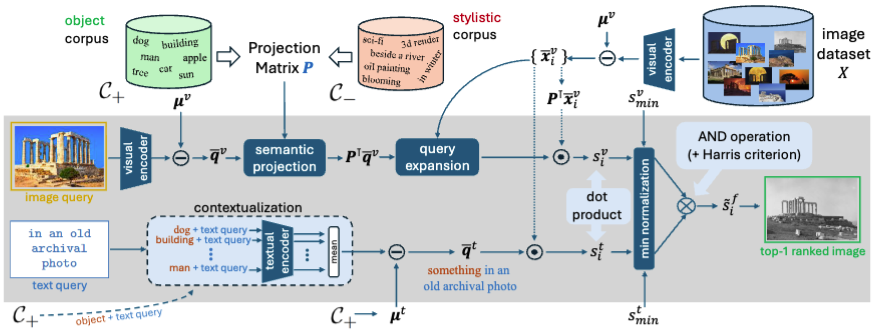
\includegraphics[width=\linewidth]{figures/basic_method}
  \caption{%
    Overview of the \textsc{Basic} post-processing pipeline.
    The image branch (top) applies centering, semantic projection, and
    query expansion; the text branch (bottom) applies centering and
    corpus contextualization. The two similarity scores are then
    normalised and combined by the Harris-inspired criterion
    (Section~\ref{sect:rel_basic_harris}).
    Reproduced from Psomas~et~al.~\cite{psomas2025icir}.%
  }
  \label{fig:basic_pipeline}
\end{figure}

\subsection{Fusion Design: a Soft Logical \textsc{and}}\label{sect:rel_basic_fusion}

The foundational idea in \textsc{Basic} is how the two modalities are combined.
Because the correct target must simultaneously respect the reference image's
visual identity \emph{and} the change demanded by the text, retrieval is
analogous to a logical \textsc{and}: an image is a good candidate only if it
satisfies \emph{both} conditions. This favours a \emph{multiplicative} combination
of the two similarity scores over an additive one. Adding the scores would reward
an image that is very strong on one modality even when it is weak on the other --
precisely the behaviour that promotes the hard negatives of
Section~\ref{sect:method_problem} -- whereas multiplying forces \emph{both} scores
to be non-negligible for the product to be large.

Concretely, for each database image \textsc{Basic} computes an image similarity
$\sv(\xdb)$ and a text similarity $\st(\xdb)$ in the shared embedding space and
combines them multiplicatively. Several post-processing steps -- centering,
semantic projection, query expansion, text contextualization, and score
normalisation -- refine these two scores before they are fused. Each is described
in turn below, and each is a candidate the method of Chapter~\ref{chapt:method}
either keeps, tunes, or supersedes; the empirical contribution of every step is
quantified in Chapter~\ref{chapt:results}.

\subsection{Centering}\label{subsect:method_centering}

Raw embeddings from a vision--language model carry a shared, uninformative
component: the ``average'' image embedding encodes generic visual patterns
(background, lighting, typical composition) and the ``average'' text embedding
reflects the statistics of everyday captions rather than any specific content.
This common component inflates all pairwise similarities and blurs the
distinctions that retrieval depends on.

\textsc{Basic} removes it by \emph{mean-centering} every feature before anything
else -- subtracting a precomputed mean vector and re-normalising, as defined in
Equation~\eqref{eq:centering} of Chapter~\ref{chapt:background}. For images the
mean $\bm{\mu}^{v}$ is estimated once on a one-million-image sample of
LAION~\cite{schuhmann2022laion5b}, a large and domain-diverse reference set, and
subtracted from the query image and every database image. For text the mean
$\bm{\mu}^{t}$ is estimated on a predefined corpus of generic object names. An
alternative is to estimate the image mean from the retrieval database itself (the
\emph{global} mean) rather than from LAION; whether the source of the mean matters
in practice is a question we answer empirically in
Section~\ref{sect:res_centering}. Because both means are computed once on fixed
corpora, centering adds no cost at query time and scales to arbitrarily large
databases.

\subsection{Semantic Projection}\label{sect:rel_basic_proj}

CLIP image embeddings mix \emph{object} information (what the thing is) with
\emph{style} information (viewpoint, lighting, background, artistic rendering). For
instance-level retrieval this is a problem, because the correct target must share
the object's identity, yet the very modifications the benchmark uses -- ``as a
sketch'', ``at night'' -- deliberately change the style. Style dimensions can
therefore drown out the identity signal. \textsc{Basic} counteracts this by
projecting the centered image features onto a subspace that \emph{emphasises
object content and suppresses style}.

The subspace is built from two small text corpora: an \emph{object} corpus
$\mathcal{C}^{+}$ of object-oriented nouns (e.g.\ ``building'', ``dog''), and a
\emph{style} corpus $\mathcal{C}^{-}$ of stylistic and contextual terms (e.g.\
``cartoon'', ``aerial view'', ``in a cloudy day''). Inspired by the
parts-of-speech-grounded subspaces of Oldfield~et~al.~\cite{oldfield2023pos},
from their centered text embeddings a weighted \emph{contrastive covariance}
matrix is formed,
\begin{equation}\label{eq:basic_proj}
  \mathbf{C}
  = (1-\alpha)\,\mathbf{C}^{+} - \alpha\,\mathbf{C}^{-},
  \qquad
  \mathbf{C}^{\pm}
  = \frac{1}{|\mathcal{C}^{\pm}|-1}
    \sum_{x\in\mathcal{C}^{\pm}}
    (\enct(x)-\bm{\mu}^{t})(\enct(x)-\bm{\mu}^{t})^{\!\top},
\end{equation}
where $\alpha$ balances the two terms. The top $k$ eigenvectors of $\mathbf{C}$ --
the directions of high variance among object words and low variance among style
words -- form a projection matrix $\mathbf{P}\in\mathbb{R}^{d\times k}$, and
centered image features $\bar{x}^{v}$ are projected as
$\mathbf{P}^{\!\top}\bar{x}^{v}$. The effect is to keep the object-semantic
directions and discard the stylistic ones. Crucially the corpora need not match
the retrieval domain -- even generic ImageNet~\cite{deng2009imagenet} class
names transfer well -- because CLIP's stylistic directions are largely
domain-independent. In practice only the
query-side image is transformed; the projection of a database image follows
implicitly from the bilinear form
$\bar{q}^{v\top}\mathbf{P}\mathbf{P}^{\!\top}\bar{x}^{v}$, so the stored database
index never has to be modified.

\subsection{Text Query Contextualization}\label{sect:rel_basic_context}

CLIP's text encoder was trained on full image captions, not on terse attribute
fragments. A bare modification text such as \emph{``make it red''} or
\emph{``during sunset''} is therefore out-of-distribution: the encoder has no way
to know \emph{what} the phrase refers to, and embeds it poorly. \textsc{Basic}
\emph{contextualizes} each modification by wrapping it in object names. For a set
of terms drawn from the object corpus $\mathcal{C}^{+}$ it builds phrases with the
object name prepended and appended (\emph{``dog during sunset''}, \emph{``sunset
dog''}, and so on), embeds all of them, centers them, and averages the result into
a single, more robust text feature. Averaging over many such fillers approximates
how CLIP would read the modification if it appeared inside a natural caption,
substantially improving the text side of retrieval. \textbf{This is the single
component that the method of Chapter~\ref{chapt:method} replaces}: instead of
padding the fragment with random nouns, it generates a full, self-contained
description of the intended target.

\subsection{Image Query Expansion}\label{sect:rel_basic_qe}

Instance retrieval often improves with \emph{query
expansion}~\cite{chum2007totalrecall,gordo2020attqe}: after an initial search,
the query is nudged towards the images it already retrieved with high
confidence, pulling it into the dense cluster of relevant items. \textsc{Basic}
uses an \emph{$\alpha$-weighted} variant that blends the query image feature with
its own top-ranked database neighbours, weighting each neighbour by how similar it
was~\cite{gordo2020attqe}. The expanded query then replaces the original for
the final image-similarity computation. As the ablation below shows, this step is
optional and its benefit on the instance-level benchmark is marginal.

\subsection{Score Normalisation and the Harris Criterion}\label{sect:rel_basic_harris}

Before fusion the two raw similarity scores $\sv$ and $\st$ live on different
scales, because the image and text branches use differently processed features. So
that neither branch dominates by accident, each score is \emph{min-normalised}: a
minimum similarity value $s_{\min}<0$ is estimated once on a held-out set and used
to shift and rescale the score so that the minimum maps to $0$,
\begin{equation}\label{eq:basic_minnorm}
  \tilde{s} = \frac{s - s_{\min}}{|s_{\min}|},
\end{equation}
after which any remaining negative residual is clamped to zero. The normalised
scores are then fused by a criterion inspired by the Harris corner
detector~\cite{harris1988corner},
\begin{equation}\label{eq:basic_harris}
  \tilde{s}^{f}
  = \tilde{s}^{v}\,\tilde{s}^{t}
  - \lambda\big(\tilde{s}^{v} + \tilde{s}^{t}\big)^{2}.
\end{equation}
The first term $\tilde{s}^{v}\tilde{s}^{t}$ is the multiplicative \textsc{and}
that rewards images relevant to \emph{both} modalities; the subtracted penalty
$\lambda(\tilde{s}^{v}+\tilde{s}^{t})^{2}$ suppresses candidates that are very
strong on one modality but only average on the other -- exactly the single-modality
false positives the benchmark is built around, and directly analogous to how the
Harris detector penalises responses dominated by a single edge direction. The
scalar $\lambda$ is fixed across all experiments.
Figure~\ref{fig:harris_surface} visualises the resulting scoring surface.

\begin{figure}[htbp]
  \centering
  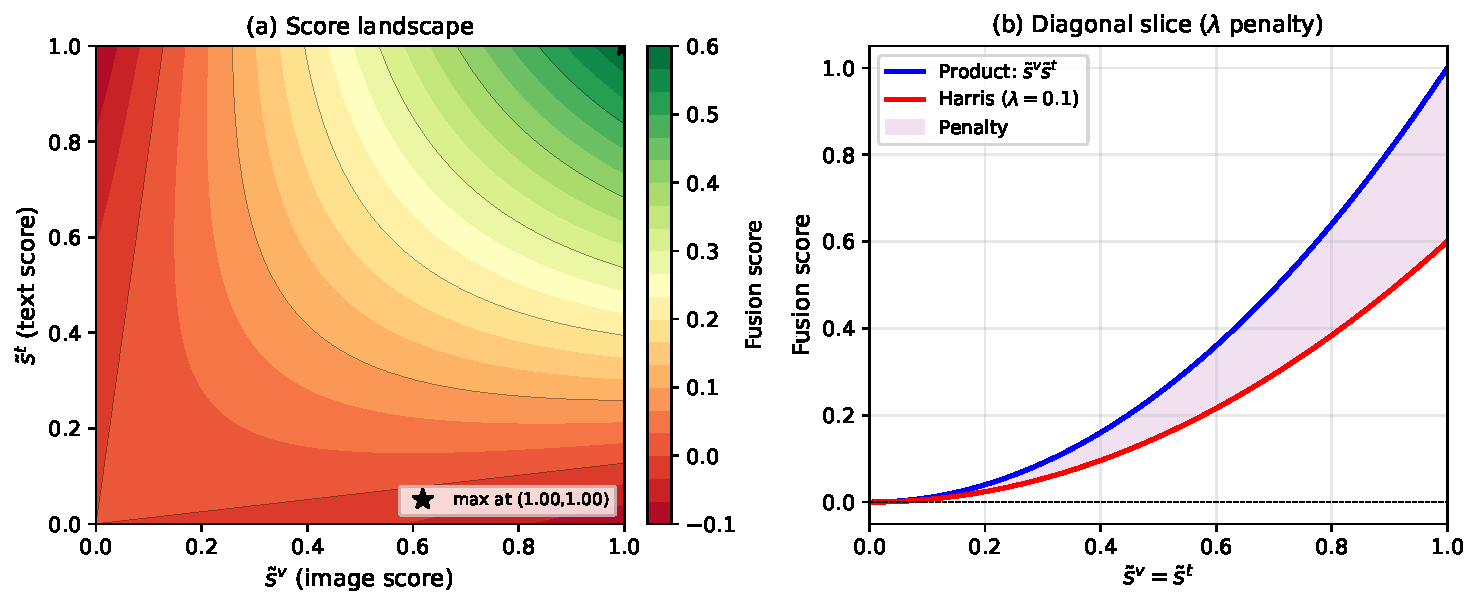
\includegraphics[width=\linewidth]{figures/harris_surface}
  \caption{%
    Response surface of the Harris fusion criterion
    $\tilde{s}^{v}\tilde{s}^{t} - \lambda(\tilde{s}^{v}+\tilde{s}^{t})^{2}$
    for $\lambda=0.1$.
    \emph{Left}: filled contour over the full $[0,1]\times[0,1]$ domain of
    normalised scores; high values (green) require both $\tilde{s}^{v}$ and
    $\tilde{s}^{t}$ to be simultaneously large.
    \emph{Right}: diagonal slice ($\tilde{s}^{v}=\tilde{s}^{t}$) comparing the
    plain product with the Harris criterion; the shaded region is the penalty
    subtracted from the product.%
  }
  \label{fig:harris_surface}
\end{figure}

\subsection{Ablation of Components}\label{sect:rel_basic_ablation}

Table~\ref{tab:basic_ablation} quantifies what each step contributes, by starting
from a plain product of raw similarities and adding components one at a time.
Reading it top to bottom tells the story of the pipeline. The bare product of raw
cosine similarities scores only $17.48\%$; \emph{centering} alone lifts this by
almost eleven points, confirming that the shared uninformative component was a
major obstacle. Score normalisation and the Harris criterion hold the score near
$28\%$. \emph{Text contextualization} then provides the single largest jump, to
$33.48\%$ -- strong evidence that the terse modification text is the principal
bottleneck of the pipeline. Semantic projection adds a further $0.87$ points to
the paper's best of $34.35\%$, while query expansion slightly \emph{reduces}
performance at the instance level (its expanded neighbours introduce more noise
than signal). Our own re-run of the released code tracks these numbers closely;
the small residual gap (at most $1.3$ points) comes from the random sampling in
the contextualization step, which draws fresh object names per query.

\begin{table}[htbp]
  \centering
  \caption{%
    Step-by-step ablation of \textsc{Basic} on i-CIR with CLIP ViT-L/14
    (macro-averaged mean average precision, \%).
    \emph{Paper}: numbers reported by Psomas~et~al.~\cite{psomas2025icir};
    \emph{Reproduced}: our re-run of the released code.%
  }
  \label{tab:basic_ablation}
  \begin{tabular}{lcc}
    \toprule
    Configuration & Paper (\%) & Reproduced (\%) \\
    \midrule
    Image$\times$Text product (baseline)      & 17.48 & 17.95 \\
    $+$~Centering                             & 28.33 & 27.76 \\
    $+$~Score normalisation                   & 27.30 & 27.40 \\
    $+$~Harris criterion                      & 28.42 & 28.33 \\
    $+$~Text contextualization                & 33.48 & 32.25 \\
    $+$~Semantic projection                   & 34.35 & 32.48 \\
    $+$~Query expansion (full \textsc{Basic})  & 31.64 & 30.28 \\
    \bottomrule
  \end{tabular}
\end{table}

The ablation reveals a clear hierarchy of importance:
text contextualization $\gg$ centering $>$ Harris normalisation
$\gtrsim$ semantic projection $\geq$ query expansion. The lesson that drives this
thesis is the size of the first gap: the \emph{textual} channel is the pipeline's
weakest link, and the largest single improvement in the whole of \textsc{Basic}
comes from making the text query easier for the encoder to read. This is exactly
the component the proposed method targets, replacing the padded fragment of
contextualization with a richer, model-generated description of the intended
target.

\paragraph{Efficiency.}
Finally, the entire pipeline is (deep-network) training-free and scales
near-linearly with the database, because scoring reduces to inner products that
off-the-shelf similarity-search libraries handle efficiently. Centering and
projection can be folded into the query side and applied on the fly over a stored
index of \emph{raw} features, so the mean and the projection matrix can be swapped
-- for instance with domain-specific knowledge -- without ever rebuilding the
index. This makes \textsc{Basic} well suited to large-scale deployment with no
adaptation, fine-tuning, or backpropagation, and the method of
Chapter~\ref{chapt:method} inherits the same property.
